%        File: COMP3121Ass1.tex
%     Created: Sun Mar 20 06:00 PM 2016 A
% Last Change: Sun Mar 20 06:00 PM 2016 A
%
\documentclass[11pt, a4paper]{article}
\usepackage{listings}
\usepackage[margin=0.8in]{geometry}
\usepackage{amsmath}
\usepackage{fancyhdr}
\usepackage{graphicx}
\pagestyle{fancy}
\title{COMP3121 Assignment 4}
\author{Alex Nguyen z3379933}
\date{15/05/16}
\lhead{Alex Nguyen z3379933}

\begin{document}
\maketitle{\textbf{Question 1)}}

\vspace{2mm}
\textit{You are running a dating agency and have m guys and f girls as customers. Each guy
and each girl have reviewed all profiles of the candidates of opposite sex and have
sent you their corresponding lists of people whose profiles they liked. Your task is to
organise a largest possible number of first dates so that everyone meets at most one
person of opposite sex and so that both parties liked each others profile (i.e., have
included the other party on their list of people whose profile they liked).
}


\vspace{5mm}

Model dating matches as a bipartite graph $G$ to whose flow is to be maximised.

Let $G$ be comprised of 2 bipartite sections of nodes $u \in L$ (males to be
matched) and nodes $v \in R$ (females to be matched).


\begin{figure}[ht!]
\centering
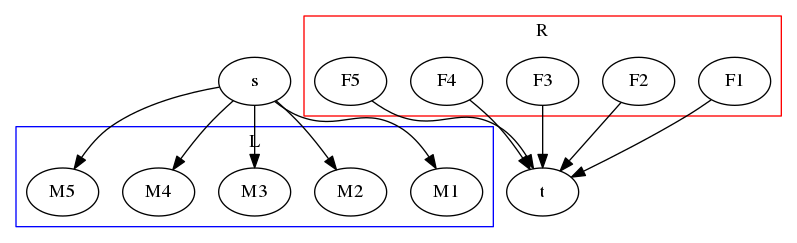
\includegraphics[scale=0.5]{q1empty.png}
\caption{Graph G augmented with sink $s$ and source $t$\label{overflow}}
\end{figure}

We populate G paths by adding edge $c(u, v)$ if node $u$ has indicated that they like
$v$'s profile and repeating for the list from both sexes for all $u \in L$ and
$v \in R$. Diagrams below show example with 5 Males, 5 Females with sample
preferences.

We now need to model the system as a flow system by adding sink $s$ and source
$t$ to graph $G$ to create $G'$.
This is represented mathematically below:
\[ G' = (V', E')\]

Where: 
\[V' = V \cup {s,t}\] 

\hspace{30mm}$E' = E$ augmented with edges from $s$ to every $u
\in L $ and every $v \in R$ to $t$.

 As each person can only be matched to one other, we represent a match in
 binary: $c(u, v) = 1$ for all $(u, v) \in E'$
 
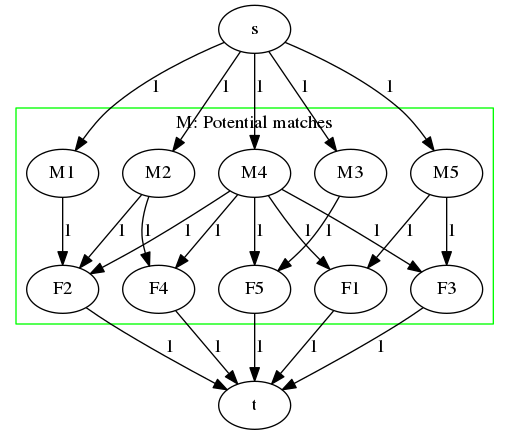
\includegraphics[scale=0.5]{q1matchset5.png}

In other words, there can be a max flow of 1 flow through each match edge
between $u$ and $v$ - when that capacity is taken, the edge is part of the max
flow scenario: matches can then be given by edges $\in M$.

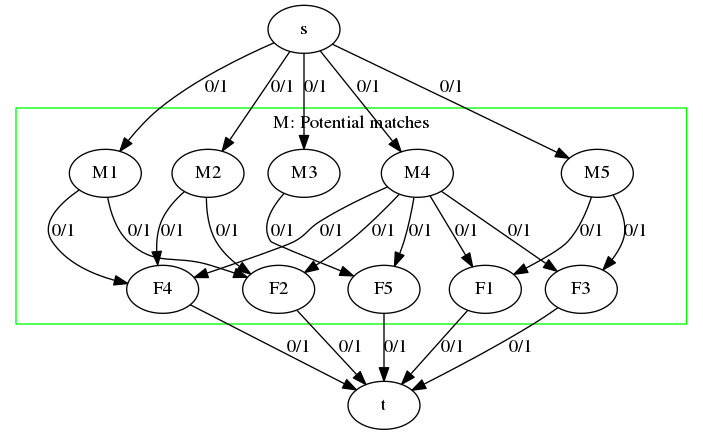
\includegraphics[scale=0.5]{q1matchset3.png}

In the figure above, we see that the maximum flow (and hence maximum match)
scenario occurs when the graph has no augmenting path and has highest number of
edges in $M$ 'switched on'.

To solve the matching problem, we use Ford-Fulkerson method/algorithm to find
max flow throughout $G'$ to find $M \subseteq E'$ such that $M$ is maximised. In
other words, pick as many edges from the list populated in $G$ such that all
picked edges are unique. The result from this will be as required (the graph was
built from mutually liked profiles, each edge in $M$ is a unique match - i.e.
one person meeting at most one other of the opposite sex). Figures 2 and 3
below show the first stages and possible augmenting path  taken by the
Ford-Fulkerson method.


\begin{figure}[ht!]
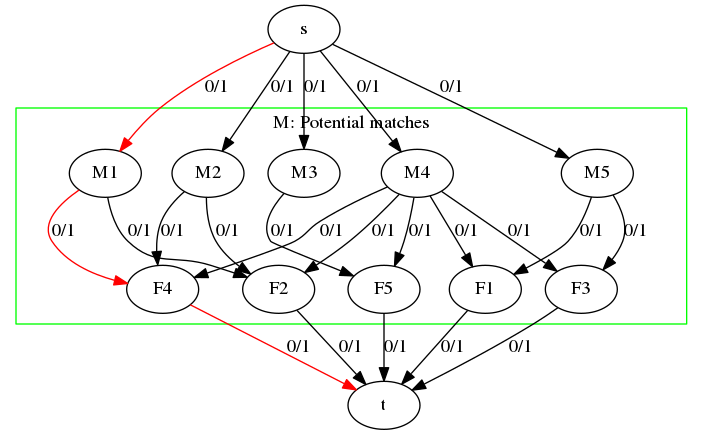
\includegraphics[scale=0.4]{q1matchset4.png}
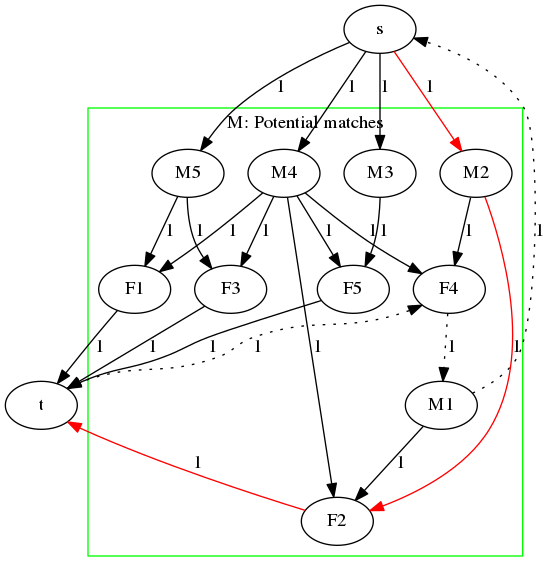
\includegraphics[scale=0.4]{q1matchset6.png}
\caption{Left - G' before applying augmented path, Right - Residual network
  $G_f$ after}
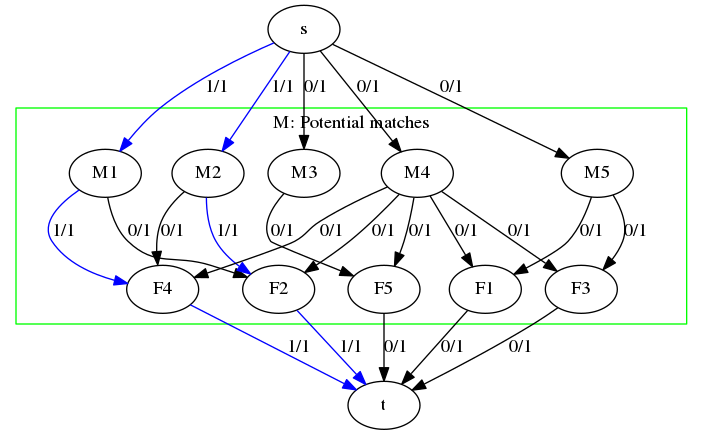
\includegraphics[scale=0.5]{q1matchset7.png}
\caption{G' after applying first 2 augmenting paths}
\end{figure}

Repeat augmentation process until no more paths from $s$ to $t$ are
possible - (occurs when augmenting $G_f$ has no edges from $s$; all pipes are
from $u \in L$ to $s$)

The above stage will generate a new augmenting path which will be repeatedly
taken until no further augmenting paths exist. As all edges have capacity of 1,
Ford-Fulkerson is an appropriate algorithm (Edmondson-Karp not needed) as
augmenting paths can only be taken once
The above stage will generate a new augmenting path which will be repeatedly
taken until no further augmenting paths exist. As all edges have capacity of 1,
Ford-Fulkerson is an appropriate algorithm (Edmondson-Karp not needed) as augmenting
paths can only be taken once. The pseudocode is shown below (from CLRS textbook)

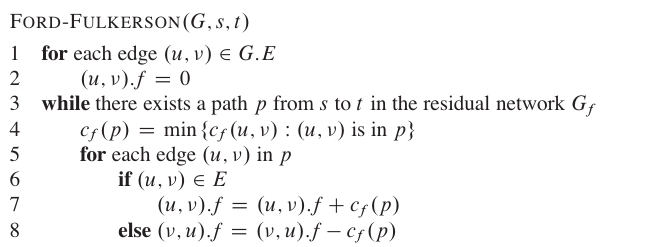
\includegraphics[scale=0.5]{ffmethod.png}

Using the Ford-Fulkerson Algorithm, we achieve a complexity of $O(Ef^{*})$, where
$E$ is as above and $f^{*}$ represents the maximum flow in graph $G$.
However, in the maximum bipartite matching case: 

$E' = O(E)$ as there are no more than edges containing nodes in $V$ are used

$f^{*} = O(V)$ as edges all have 1 capacity - edges only can be turned on or off
so augmenting paths can only be used once each. In other words, they are bounded
by $min(|L|, |R|)$

Hence, the matching algorithm will complete in $O(VE)$ time.

\maketitle{\textbf{Question 2)}}

\textit{Design an algorithm for determining which cables to disconnect to
  isolate computers $Q_{1} ... Q_{m}$ for all computers $P_{1} ... P_{n}$ so 
that the total cost incurred is minimal}


\vspace{35mm}
\maketitle{\textbf{Question 3)}}

\textit{Design an algorithm which, given a flow network, finds a minimal cut in the network and which runs in polynomial time. Can there be more than one minimal cut? If so give an example of a flow network with more than one minimal cut.}

\vspace{2mm}
\vspace{40mm}
\maketitle{\textbf{Question 4)}

\textit{You work for a new private university which wants to keep the sizes of classes small.
Each class is assigned its maximal capacity - the largest number of students which
can enrol in it. Students pay the same tuition fee for each class they get enrolled
in. Students can apply to be enrolled in as many classes as they wish, but each of
1
them will eventually be enrolled to at most 5 classes at any given semester. You are
given the wish lists of all students, containing for each student the list of all classes
they would like to enrol this particular semester and you have to chose from the
classes they have put on their wish lists in which classes you will enrol them, without
exceeding the maximal enrolment of any of the classes and without enrolling any
student into more than 5 classes. Your goal is, surprisingly, to maximise the income
from the tuition fees for your university. Design an efficient algorithm for such a task} 

Similar to \textbf{Question 1}, we model the scenario using a bipartite graph
and take the maximum flow to maximise classes enrolled in by students.
This will maximise tuition fees and hence income to the university.

The graph G will show which students will end up matched to which class
In this case, $u \in L$ will be comprised of students and $v \in R$ will
represent each class to be chosen. However, as there are max 5 allowed classes per
student and classes have a maximum capacity (which differs per available class)
differ. %Graph with 5 from source, cap_i to sink

\vspace{2mm}


\maketitle{\textbf{Question 5)}}

\textit{Assume each student can borrow at most 10 books from the library, and the library has three copies of each title in its inventory. Each student submits a list of books he wishes to borrow. You have to assign books to students, so that a maximal number of volumes is checked out}.
\vspace{4mm}

Similar to \textbf{Question 1}, we model the scenario using a bipartite graph
and take the maximum flow to see maximum parallel books borrowed by each
student (hence max volumes checked out). 
The max flow will show which books are matched to which student.
In this case, $u \in L$ will be comprised of students and $v \in R$ will
represent individual books to be chosen. However, as there are 3 copies
of each book and students are restricted to 10 books each, edge capacities will 
differ. %Graph with 10 from source, 3 to sink

\vspace{50mm}

\maketitle{\textbf{Question 6)}}
\textit{The emergency services are responding to a major earthquake that has hit a wide region, and left n people injured who need to be sent to a hospital. Let P be the set of n people and H be the set of k hospitals. Several hospitals are available to treat these people, but there are some constraints:} \vspace{2mm}

\textit{(a) Each injured person needs to be sent to a hospital no further than one hour drive away. Let $Hp$ be the set of hospitals that are within range for person $p$.}

\textit{(b) Each hospital h has a capacity $ch$ , the maximum number of people that the hospital can receive.}

\textit{Develop an efficient algorithm that determines whether it is possible to assign each person to a hospital in a way that satisfies these constraints, and returns such an assignment if so.}

\end{document}
